\begin{ejercicio}[
  id=CAL_FUN_001,
  materia=calculo,
  capitulo=funciones,
  nivel=intermedio,
  procedencia="Libro Cálculo Avanzado",
  visibilidad=true,
  libros={calculo1, calculo_avanzado},
  youtube_url="https://www.youtube.com/watch?v=ejemplo_calculo",
  mostrar_solucion=true,
  libro_promocion=""
]
Considera la función $f(x) = x^3 - 3x + 1$. Determina los puntos críticos y clasifícalos como máximos, mínimos o puntos de inflexión.

\textbf{Nota:} Utiliza la gráfica de la función para visualizar los puntos críticos.

\begin{figure}[h]
\centering
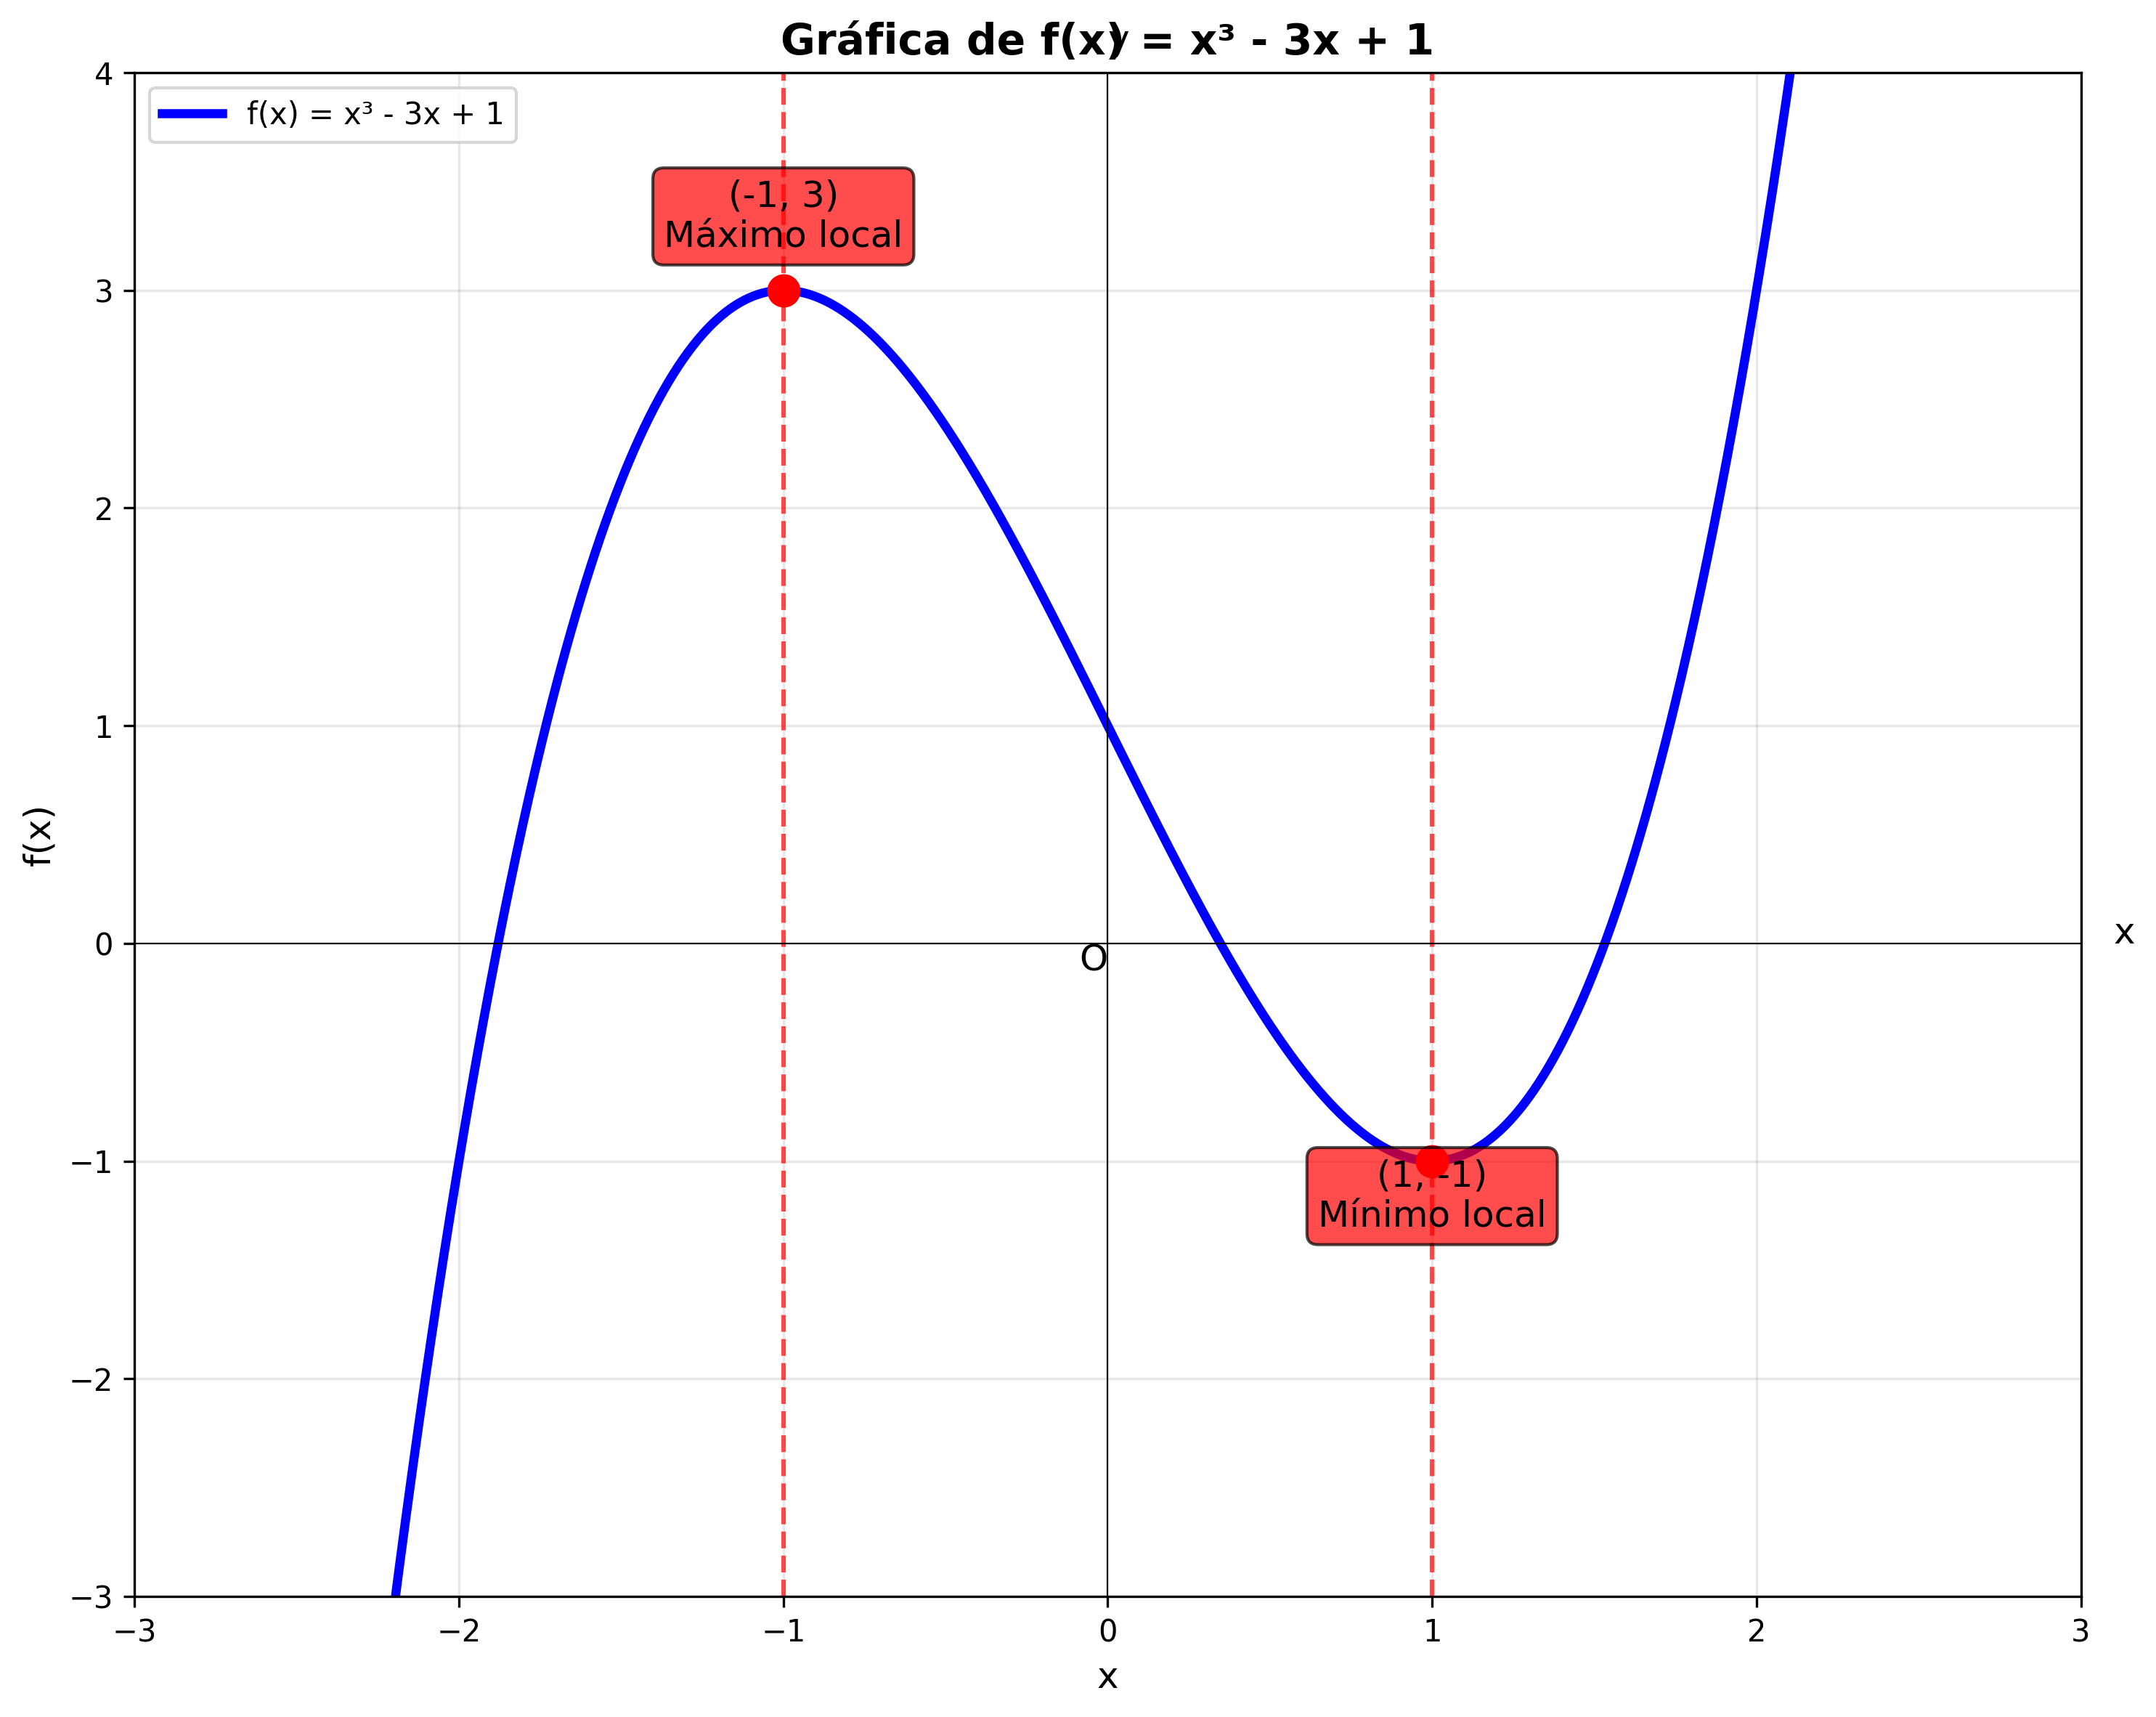
\includegraphics[width=0.8\textwidth]{imagenes/funcion_cubica_001.png}
\caption{Gráfica de la función f(x) = x³ - 3x + 1 con puntos críticos marcados}
\label{fig:funcion_cubica}
\end{figure}

\begin{solucion}
Para encontrar los puntos críticos, seguimos estos pasos:

1) \textbf{Calculamos la primera derivada:}
   $$f'(x) = 3x^2 - 3 = 3(x^2 - 1) = 3(x+1)(x-1)$$

2) \textbf{Encontramos los puntos críticos:}
   $$f'(x) = 0 \Rightarrow x = -1 \text{ o } x = 1$$

3) \textbf{Calculamos la segunda derivada:}
   $$f''(x) = 6x$$

4) \textbf{Clasificamos los puntos críticos:}
   \begin{itemize}
   \item Para $x = -1$: $f''(-1) = -6 < 0$ → \textbf{Máximo local}
   \item Para $x = 1$: $f''(1) = 6 > 0$ → \textbf{Mínimo local}
   \end{itemize}

5) \textbf{Calculamos los valores de la función:}
   \begin{itemize}
   \item $f(-1) = (-1)^3 - 3(-1) + 1 = -1 + 3 + 1 = 3$
   \item $f(1) = (1)^3 - 3(1) + 1 = 1 - 3 + 1 = -1$
   \end{itemize}

\textbf{Respuesta:}
\begin{itemize}
\item Punto máximo local: $(-1, 3)$
\item Punto mínimo local: $(1, -1)$
\end{itemize}

\textbf{Nota:} La gráfica muestra claramente el comportamiento de la función y confirma nuestros cálculos.
\end{solucion}
\end{ejercicio} 